\section{Neural Networks}
Motivation: train feature maps $\phi$ and weights $w$ (generally non-convex, initialization matter) $w^* = \arg \min_{w, \textcolor{blue}{\theta_j}} \sum^n_{i=1}l(y_i; \sum^m_{j=1}{w_j}{\phi(x_i;\textcolor{blue}{\theta_j})})$

\textbf{Activation functions}
1. Identity; 2. Sigmoid: $\frac{1}{1+exp(-z)}$; 3. Tanh: $\frac{exp(z)-exp(-z)}{exp(z)+exp(-z)}$; 4. ReLU: $max(0, z)$ 

%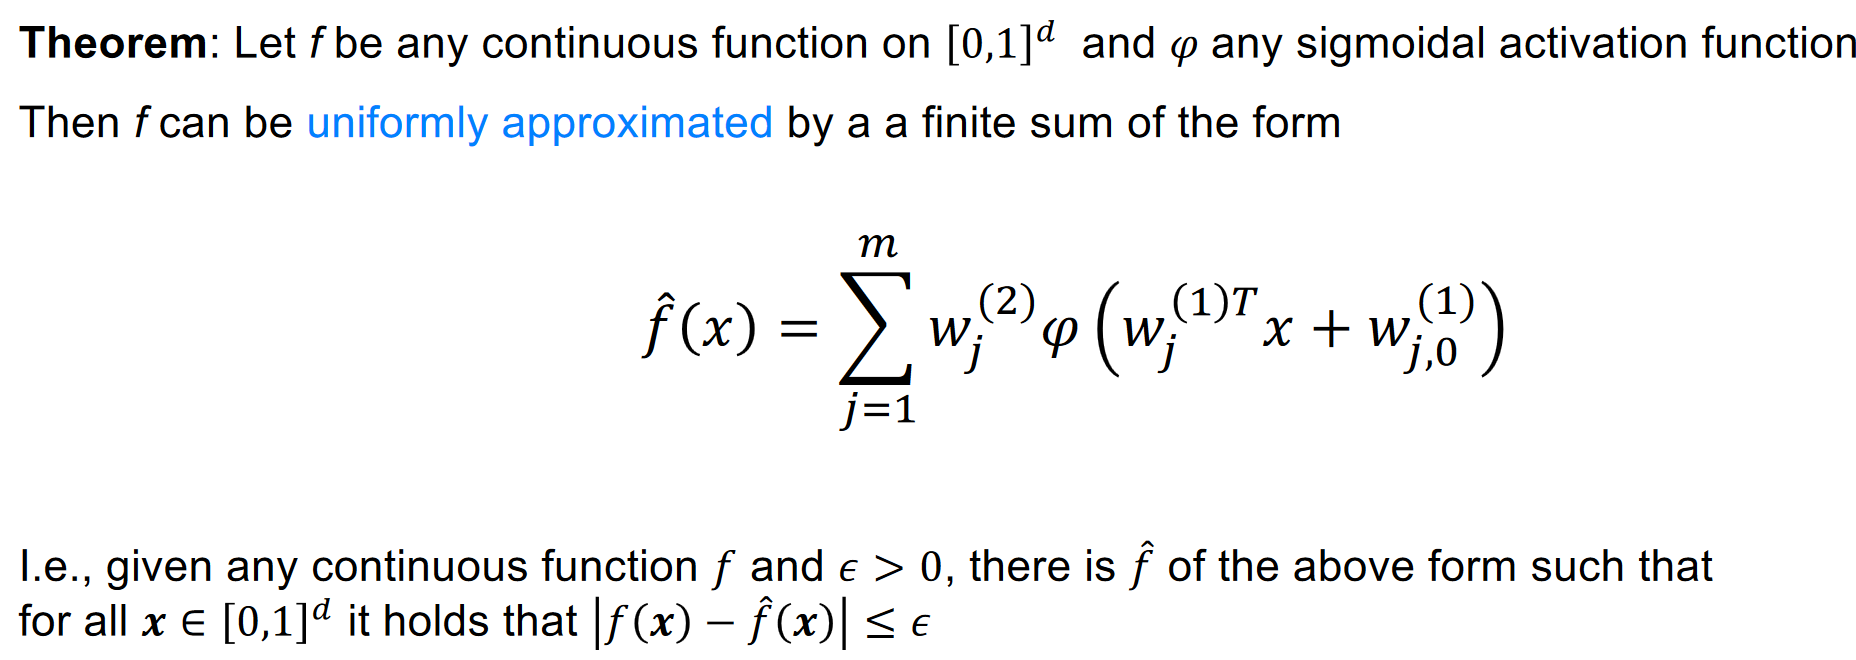
\includegraphics[width=\linewidth]{pics/figure8.PNG}
\textbf{Derivative of activation functions} \\
1. Sigmoid $\phi'(z)$ = $(1-\phi(z))\phi(z)$; 2. ReLU $\phi'(z) = 1$ if $z>0$; $0$ if $z<0$ (not differential at z=0, manually define derivative at 0 is 0)\\
\textbf{Backpropagation}
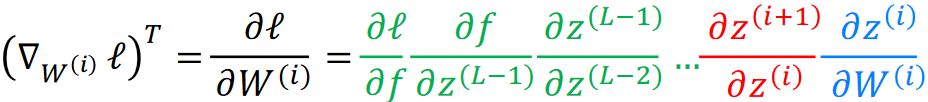
\includegraphics[width=\linewidth]{pics/figure9.PNG}
or it can rewrite into Matrix form:\\
$\nabla_{W^{(i)}}l = \delta^{(i)}\nu^{(i-1)T}$ where  error signal: \\ $\delta^{(i)} = 
\begin{cases}
\nabla_f l&, \text{output layer}\\
\varphi'(z^{(i)}) \odot (W^{(i+1)T}\delta^{(i+1)})&, \text{hidden layer}
\end{cases}$\\
and $\nu^{(i)} = \varphi(W^{(i)}\nu^{(i-1)})$\\
\textbf{Potential Issue}
Exploding or vanishing gradient (solve by using certain activation function, e.g. ReLU or keeping the magnitude of $\nu^{(i)}$)\\
\textbf{Initializing weights}
Goal: Keep variance of weights approximately constant across layers to avoid vani. and explod. grad. 
\textbf{Random initialization} 
Glorot ($tanh$), He (ReLU)
\textbf{Avoid overfitting}
Regularization (weight decay); Early stopping; Dropout p (=Pr(remain), test: $\sigma(W \times p)$)



\section{Convolutional Networks}
\textbf{CNN vs ANN}:\\
- Invariance to the augumentation of the training set\\
- Fewer parameters (parameters sharing in CNN)\\
- The weights can still be optimized via backprop.\\
\textbf{Batch normalization}:\\
1. Use on the mini-batch;\ 
2. Reduces internal covariate shift;\ 
3. Enables larger learning rates;\ 
4. Has regularizing effect
5. Solve vani./expl. grad.\\ 
1. Normalize each point with mini-batch mean and variance $\hat{x}_t = \frac{x_t-\mu_s}{\sqrt{\sigma_s^2+\epsilon}}$; 2. Scale and shift with 2 learnable parameters $\Tilde{x_t} = \gamma \hat{x_t} + \beta$
%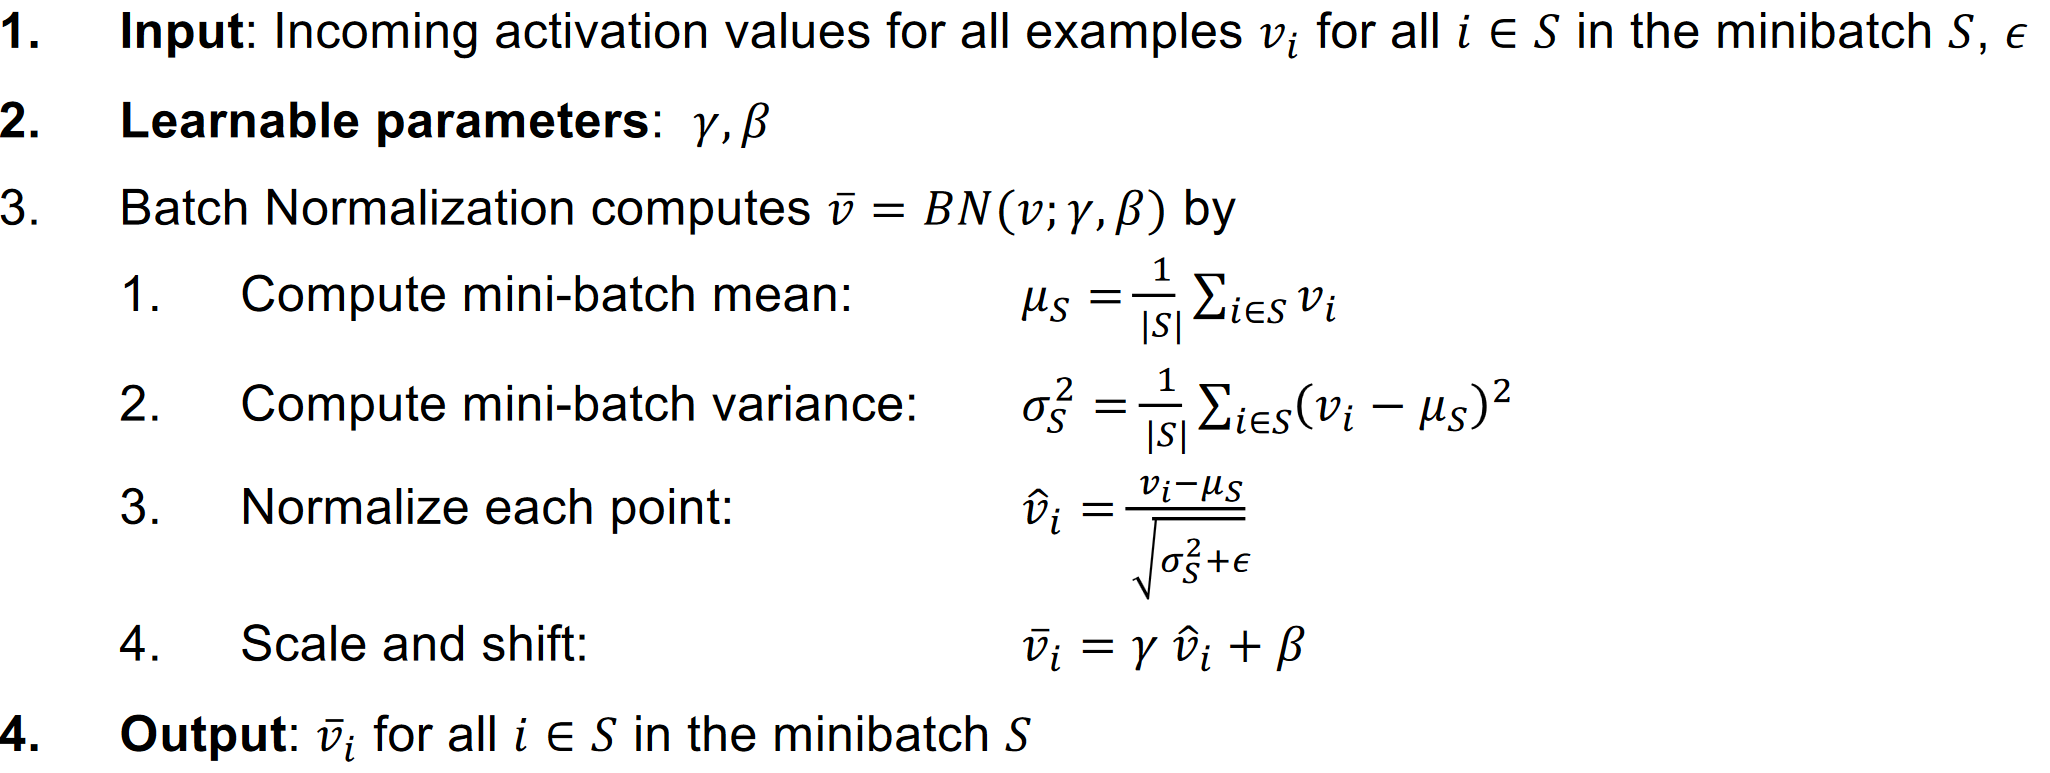
\includegraphics[width=0.9\linewidth]{pics/figure10.PNG}
\textbf{Convolutions in 1D}: 
Given vector $w \in \mathbb{R}^k$ and $x \in \mathbb{R}^d$, convolution result: $z_i = \sum^{min(i,k)}_{j = max(1, i-d+1)}{w_j}x_{i-j+1}$ \\
\textbf{Output}:
m $f\times f$ filters, a $n \times n$ image as input, padding p and stride s: output size = $\frac{n+2p-f}{s}+1$\\
\textbf{Pooling layers}:
aggregate several units (max/average) to decrease the width of the width of the network\\
\textbf{Residual Connections}
1. Skip connections for effectively training deeper networks;\quad 2. Allows identity as optimal solution (avoid vanishing gradients)
%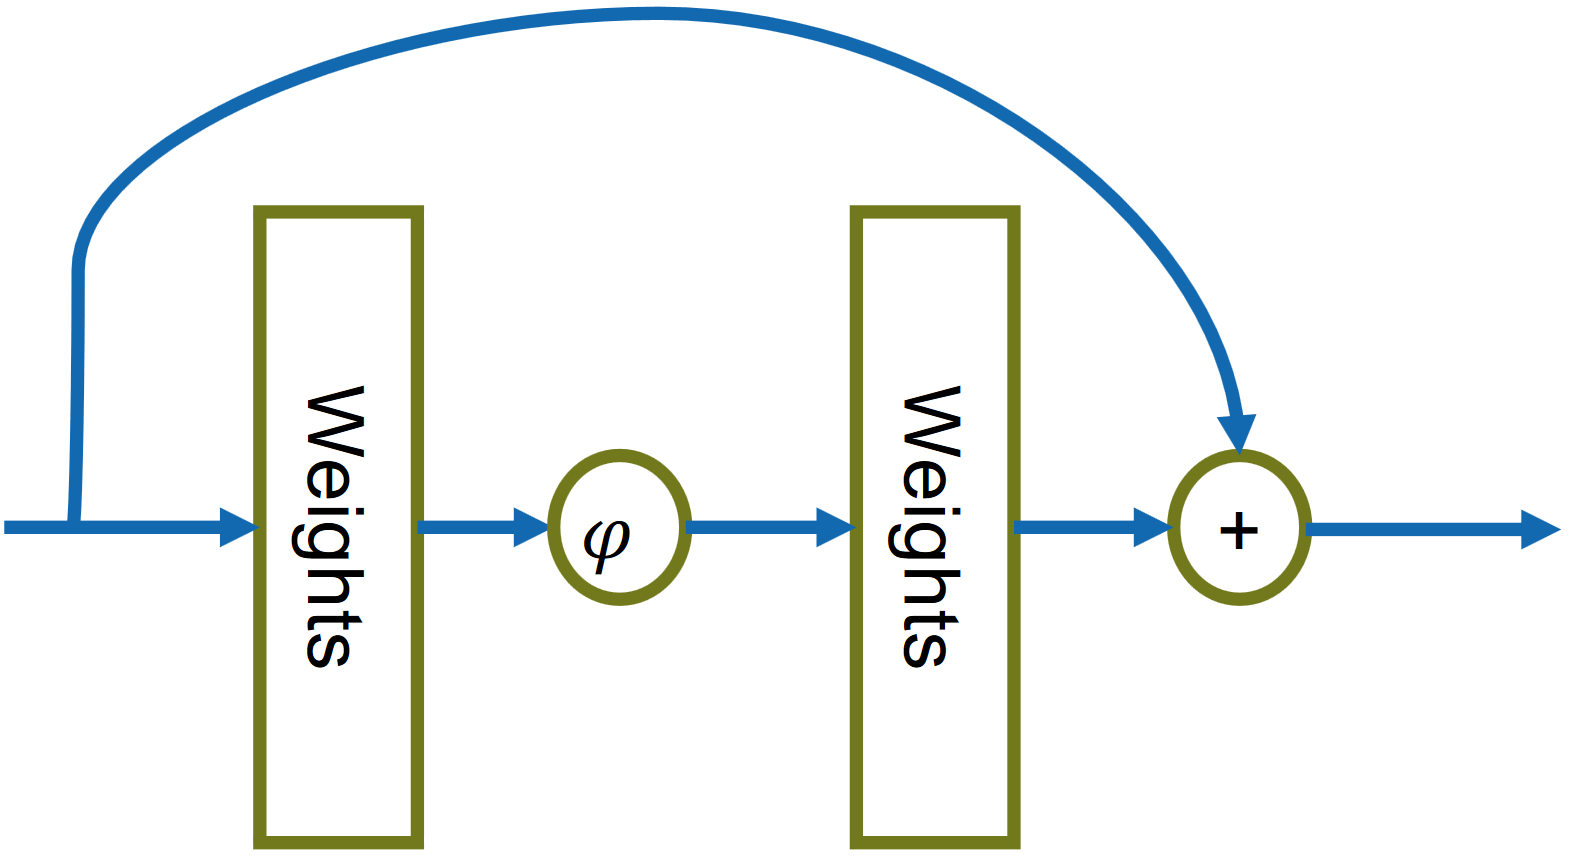
\includegraphics[width=\linewidth]{pics/figure11.PNG}
